%\subsubsection{Boson Tagger}
\label{subsec:bkg_uncer_vtagger}
For the uncertainties associated with the boson tagger's background efficiency, we consider both the large-$R$ jet-related uncertainties and the modeling uncertainties from multijet and $\gamma$+jets processes. The modeling uncertainties are estimated by comparing the nominal Pythia 8 and Sherpa samples for multijet and $\gamma$+jets, respectively, against their alternative samples. For more details on how the tagger is defined, see Section~\ref{subsubsec:merged_jets_selection}.
%\cite{ATL-PHYS-PUB-2020-017}.

Systematic uncertainties associated with the scale factors, which assess the boson tagger’s relative performance in data versus MC, are thoroughly evaluated. These uncertainties include various aspects: for background, considerations include matrix element variations, hadronization, radiation effects, and the impacts from dijets or $\gamma$+jets events. For the signal, uncertainties include considerations like extrapolation at high \pt.

Plots illustrating the impact of uncertainties on the Data/MC ratio for the \olep channel are presented in Figure \ref{fig:1LepVTaggerUnc}.

\begin{figure}[ht]
    \centering
    \begin{subfigure}[b]{0.32\textwidth}
        \centering
        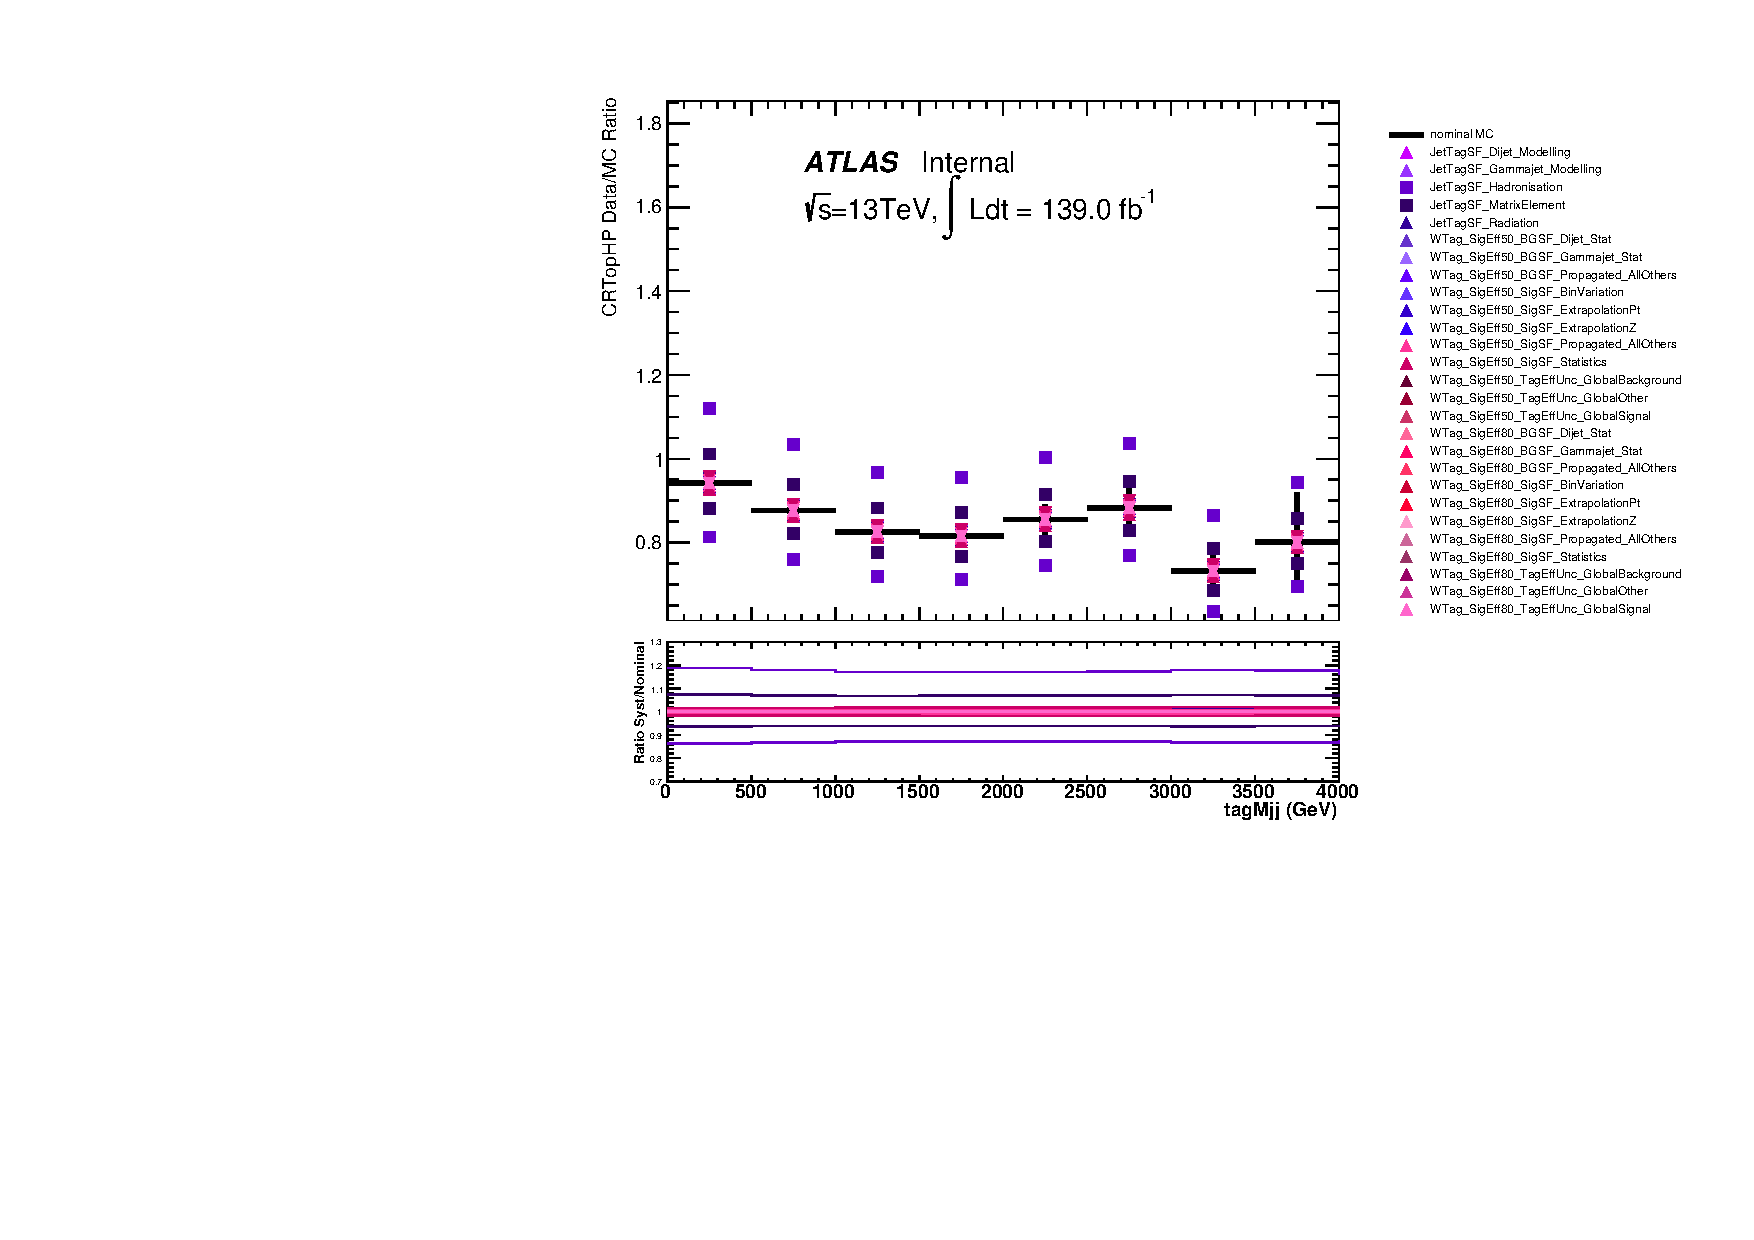
\includegraphics[width=\textwidth]{figures/1lep/VTaggerUnc/VTagCRTopHPtagMjj_SystBreakDown.pdf}
        \caption{Merged HP TopCR}
        \label{fig:MergedHPTopCR}
    \end{subfigure}
    \begin{subfigure}[b]{0.32\textwidth}
        \centering
        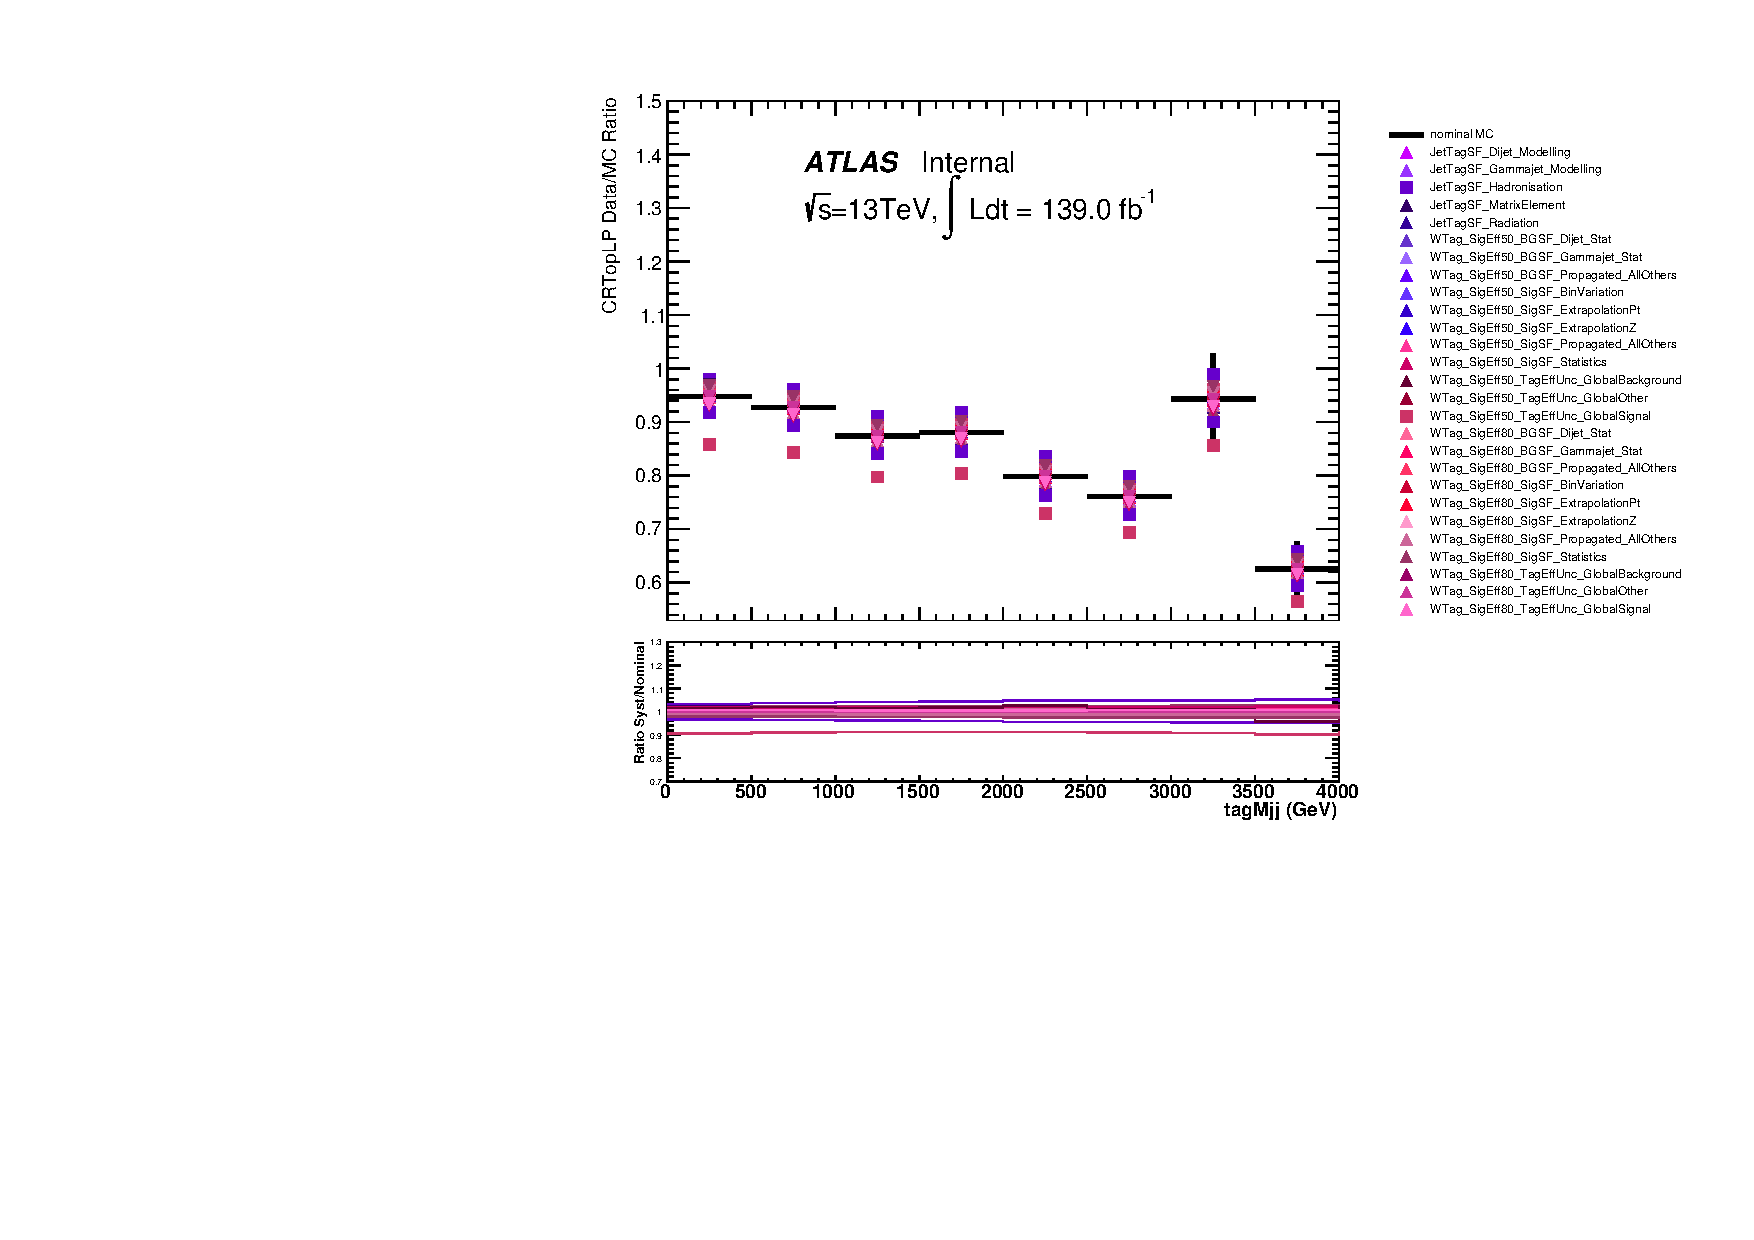
\includegraphics[width=\textwidth]{figures/1lep/VTaggerUnc/VTagCRTopLPtagMjj_SystBreakDown.pdf}
        \caption{Merged LP TopCR}
        \label{fig:MergedLPTopCR}
    \end{subfigure}
    \begin{subfigure}[b]{0.32\textwidth}
        \centering
        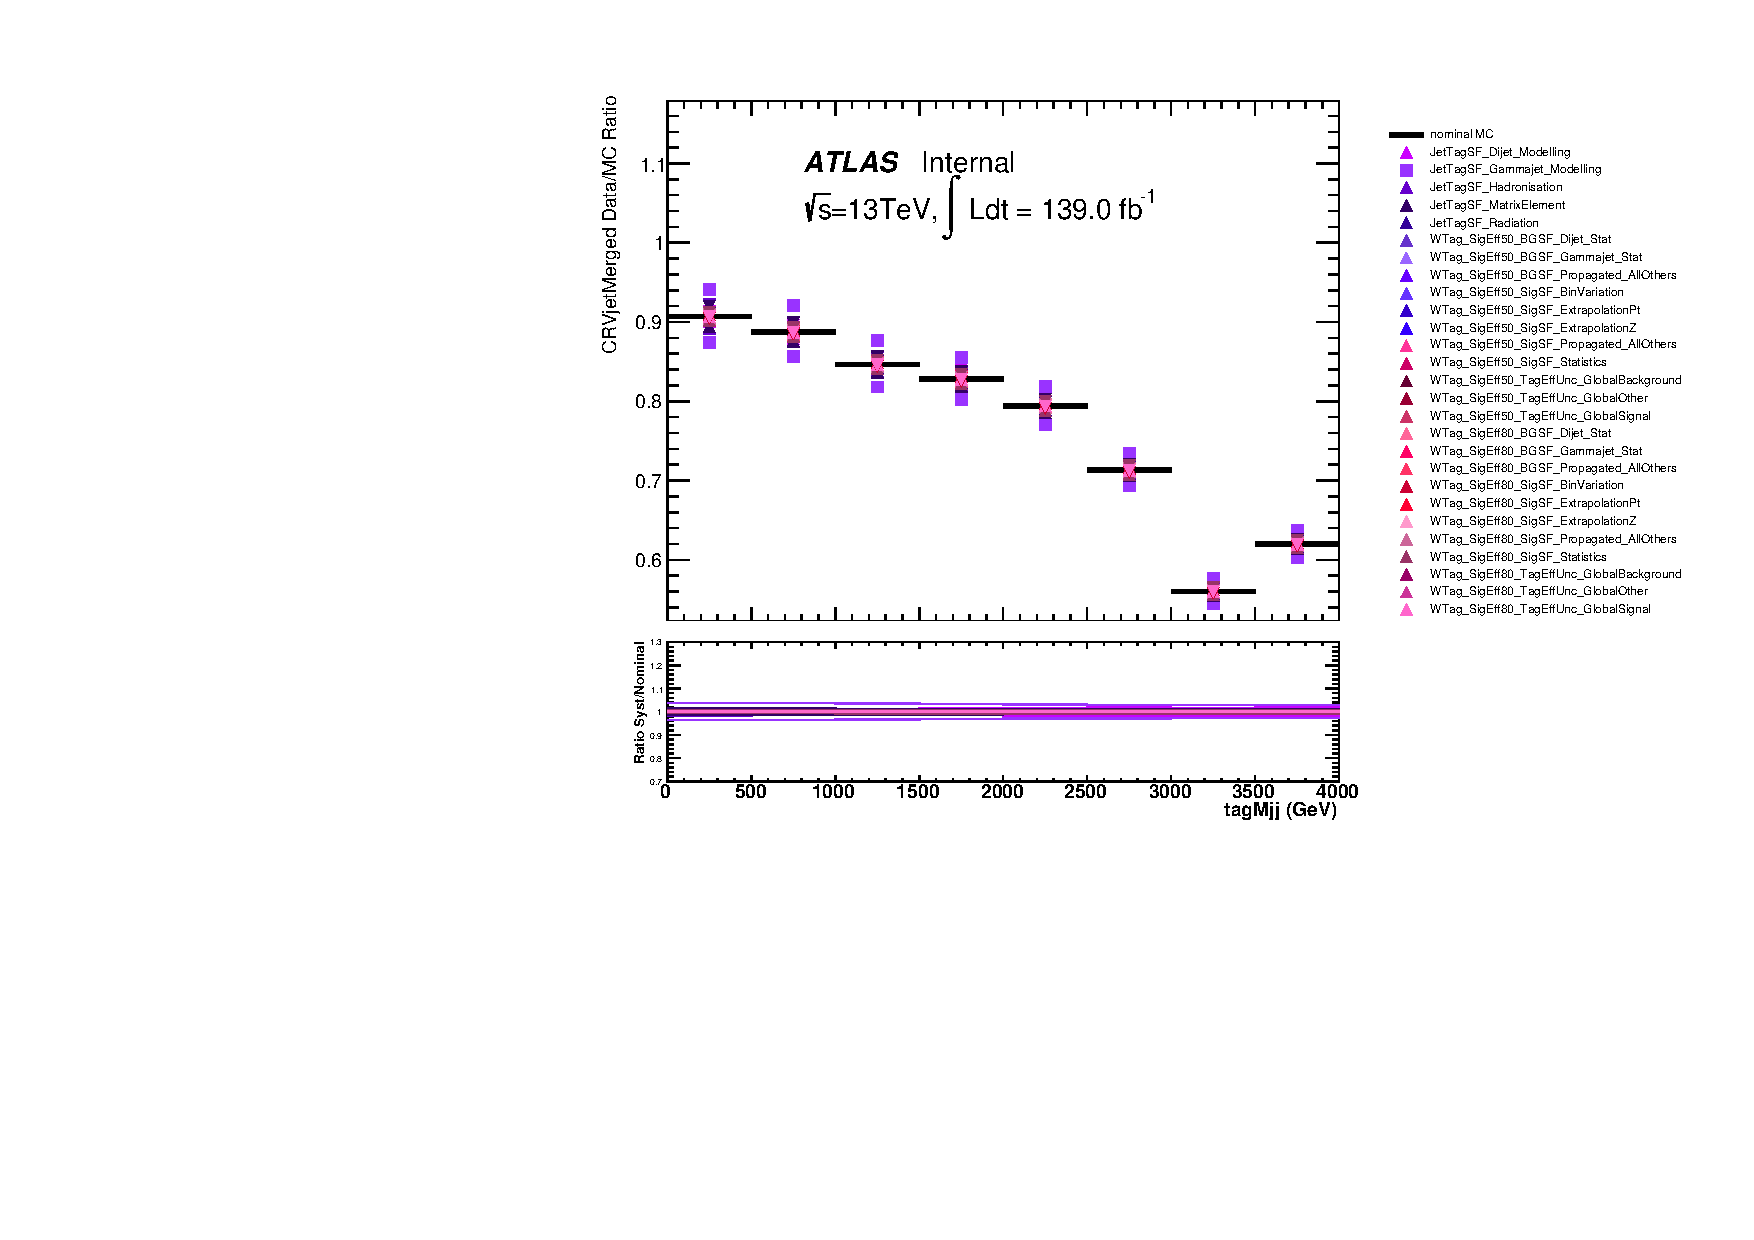
\includegraphics[width=\textwidth]{figures/1lep/VTaggerUnc/VTagCRVjetMergedtagMjj_SystBreakDown.pdf}
        \caption{Merged Wjets CR}
        \label{fig:MergedWjetsCR}
    \end{subfigure}
    \caption{Comparison of boson tagging scale factors in the 1-lepton channel.}
    \label{fig:1LepVTaggerUnc}
\end{figure}


